\chapter{Einleitung}

Im folgenden Abschnitt werden die aus technischer Sicht relevanten Aspekte genauer analysiert. Zu Beginn wird das Aufgabenumfeld in einem weiteren Sinne betrachtet, später wird konkret auf die Analyse und die Realisierung eingegangen.
\\

Der Hauptteil richtet sich vor allem an Personen, die bereits Hintergrundwissen zum Betriebssystem Android vorweisen sowie für Entwickler, die an der Weiterentwicklung des Produktes interessiert sind.

\section{BigPicture}
Zur Übersicht wird das Umfeld der Applikation in einem BigPicture zusammengefasst. Es ermöglicht die Darstellung der äusseren Einflussfaktoren sowie die Abgrenzung des Systems zu definieren.

\begin{figure}[h!]
\caption{Das Aufgabenumfeld in einem BigPicture zusammengefasst}
\centering
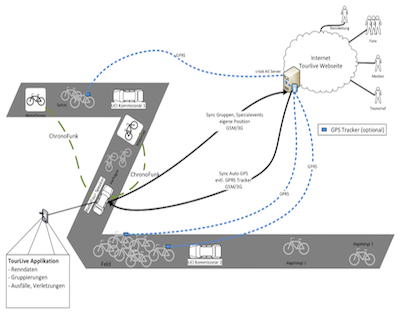
\includegraphics{05bericht/images/big_picture.png}
\end{figure} 

Die schematische Darstellung zeigt im wesentlichen die drei Hauptaktoren auf. Zum einen sind dies die Motorradfahrer, welche die Radrennfahrer begleiten und Veränderungen in Echtzeit per Funk übermitteln. Diese Informationen kommen in kurzen Abständen und müssen sofort erfasst werden können. Im UserInterface verwenden wir dafür eine Lösung bei der mehrere Radrennfahrer gleichzeitig eingetragen werden können.
\\

Eine weitere Rolle spielt der \textit{RadioTour Speaker} mit dem Android Tablet. Er fasst die Informationen zusammen und wertet diese bereits auf dem Gerät aus. Im Tablet werden auch Daten wie z.B. die Durchschnittsgeschwindigkeit und die aktuelle Rennzeit angezeigt.
\\

Der dritte Aktor bildet der Server der \textit{cnlab AG}, welcher direkt mit der Applikation kommuniziert. Ausgetauscht werden die Veränderungen im Feld sowie Rückstände von der Spitze. Weiter können Ereignisse wie z.B. eine Verletzung oder ein defektes Fahrrad aufgezeichnet werden. Die Daten werden dann weiter auf der Webseite der \textit{TourLive} aufbereitet und publiziert. Nicht nur für die beteiligten im Team sondern auch für Fans sind diese Angaben von grossem Interesse, da die Daten vor den offiziellen Zeitmessungen bereits einen Einblick in das Schlussklassement geben. Das BigPicture ist in voller grösse ebenfalls im Anhang \ref{fig:bigpicture}.

\section{Evaluation und Kaufempfehlung}
\label{kap:kaufempfehlung}
Die Evaluation der Zielplattform war ein wichtiger Faktor für die weitere Entwicklung der Arbeit. Aus diesem Grund stand dies ganz zu Beginn der Arbeit an. Zur Auswahl standen die beiden marktführenden Betriebssysteme Android (Google) und iOS (Apple). Als Grundlage für die Evaluation dienten die folgenden Kriterien:
\begin{itemize}
\item Vorkenntnisse der Programmiersprachen Java bzw. Objective-C
\item Möglichkeiten zum UserInterface Design
\item Programmierumgebung, \gls{ide}
\item mögliche Vertriebskanäle der Applikation
\item Nutzbarkeit von externen Geräten und Schnittstellen
\item Vielfalt von Informationsquellen im Internet
\end{itemize}
Die Kriterien werden in einer Nutzwertanalyse gewichtet und bewertet. Insbesondere die Vorkenntnisse in Java sind  ausschlaggebend für den Entscheid, die Applikation für die Androidplattform zu entwickeln. Dieser Entscheid ist in Absprache mit Herrn Heinzmann getroffen worden. Die gesamte Liste der Kriterien mit der jeweiligen Gewichtung sowie eine ausführliche Erläuterung befinden sich im Anhang \ref{ref_kriterien}.
\\

Für die Auswahl eines geeigneten Tablets wird im nächsten Schritt ein Kriterienkatalog definiert mit zwingenden und optionalen Kriterien für das Gerät. Die zwingenden Kriterien beinhalten:
\begin{itemize}
\item Android Betriebssystem, gemäss Evaluation
\item USB Anschluss für den Import der Fahrerliste am Renntag, optional auch mit Adapter möglich
\item Mobilfunktnetz 3G für die Kommunikation mit dem Server
\item GPS für die Lokalisierung
\item Stromversorgung durch 12V (Auto) Adapter möglich
\end{itemize}
Zu den optionalen Kriterien gehören die Akkulaufzeit, falls die Stromversorgung unterbrochen wird sowie ein grosszügiger Bildschirm für die Bedienung mit dem Finger oder mithilfe eines Stiftes.
\\

Als Sieger und somit auch als Kaufempfehlung an die \textit{cnlab AG} geht das Lenovo ThinkPad Tablet. Dieses Gerät erfüllt alle Kriterien und überzeugt in der Vielfalt der Anschlüsse. Die Kaufempfehlung mit weiteren Erläuterungen ist ebenfalls im Anhang \ref{ref_kaufempfehlung} zu finden.
\\

Im Verlauf der Arbeit ist ein defekt an der Micro USB Buchse entstanden. Dieser Anschluss wird für die Entwicklung auf dem Gerät dringend benötigt. Für die weitere Entwicklung ist ein Ersatzgerät angeschafft worden. Dabei handelt es sich um das Galaxy Nexus Tab 10.1\footnote{\url{http://www.samsung.com/ch/consumer/mobile-phone/tablets/tablets/GT-P7500UWDITV} aufgerufen am 23.05.2012}
